%% ID: metal_block
%% TITLE: A Metal Block
%% TYPE: question
%% QUESTIONTYPE: numeric
%% CONCEPTS: energy, momentum, eq_of_motion_diff
%% VIDEOS: 
%% LEVEL: 3
%% TOPIC: mechanics/dymanics
%% ORDER: 7

\begin{problem}[A1987PSIIQ9a] %Acceleration and work done problem, with some SUVAT
{A metal block of mass $m$ rests on a rough wooden surface. A thread is attached to the right side of the block and a tension is applied to cause it to move. The motion is opposed by a constant frictional force $F_{r}$ between the block and the surface.
\begin{enumerate}
	\item Draw a diagram to show all the forces on the block immediately after motion commences.
	\item When the tension in the thread is $T$, the acceleration of the block is measured to be $a$. Calculate the new acceleration, $a_{n}$, if the tension is increased to $\frac{5}{4}T$.
	\item With the tension of $\frac{5}{4}T$ applied, the block accelerates from rest but after a time $t$ the string breaks. Explain the subsequent motion of the block, and also show that it travels a total distance of \begin{equation*} s = \frac{1}{2} \left(a_{n} + \frac{a_{n}^{2}m}{F_{r}} \right)t^{2}\end{equation*} from its initial position.
	\item Given that $T = 400 \textrm{ N}$, $m = 100 \textrm{ kg}$, $t = 2 \textrm{ s}$ and $a = 0.1 \textrm{ ms}^{-1}$, calculate the work done by the block after the string breaks.
\end{enumerate}
}
{\textit{Adapted with permission from UCLES, A Level Physical Science, June~1987, Paper~2, Question~9.}}
{\begin{enumerate}
	\item Figure \ref{fig:Dynamics_block_string} is a diagram showing all of the forces acting on the block:
\begin{figure}[h]
\centering
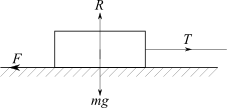
\includegraphics[width=0.4\textwidth]{Dynamics_block_string}
\caption{}
\label{fig:Dynamics_block_string}
\end{figure}
	\item This part requires only Newton's Second Law, $\vtr{F} = m\vtr{a}$. Initially we have 
	\begin{equation*} \textrm{Acceleration } = \frac{F}{m} = \frac{T - F_{\textrm{r}}}{m} = a \end{equation*}
and then the tension is increased, and so the acceleration increases to
	\begin{equation*} \textrm{New Acceleration } = \frac{F_{\textrm{new}}}{m} = \frac{\frac{5T}{4} - F_{\textrm{r}}}{m} = a + \frac{T}{4m} = a_{n} \end{equation*}
	
	\item The block will accelerate up to a maximum speed $u_{\textrm{max}} = a_{n}t$, which comes from $v= u + at$ but where $u = 0$, $a = a_{n}$, $t=t$ and $ v = u_{\textrm{max}}$ which will occur as the string breaks and the block stops accelerating. After this point the only force acting to affect the block's motion is the friction (the normal reaction and the weight are perpendicular to the motion, so do not affect it), and the block will decelerate to a halt.

To calculate the distance, we recognise that we have two periods of constant acceleration and so can use the SUVAT equations: we need to use the equations $s = ut + \frac{1}{2}at^{2}$ and $v^{2} = u^{2} + 2as$ here. The motion can be split into two sections; that with the tension, and that without; call the distance moved whilst the tension acts $s_{1}$ and the distance without $s_{2}$, we want $s = s_{1} + s_{2}$.

To find $s_{1}$ we use $s = ut + \frac{1}{2}at^{2}$, where $u = 0$, $a = a_{n}$ and $t = t$:
\begin{equation*} s_{1} = (0)t + \frac{1}{2} a_{n}t^{2} = \frac{1}{2} a_{n}t^{2} \end{equation*}

Finding $s_{2}$ is slightly more complicated, but since we worked out the speed it was moving at as the string breaks, we can use the second SUVAT equation; since we know the initial and final velocities. We have $u = u_{\textrm{max}} = a_{n}t$, $v = 0$ and also $a = \frac{-F_{r}}{m}$ from Newton's Second Law:
\begin{equation*} s_{2} = \frac{v^{2} - u^{2}}{2a} = \frac{- u_{\textrm{max}}^{2}}{2\left( \frac{-F_{r}}{m} \right)} = \frac{a_{n}^{2} t^{2} m}{2 F_{r}} \end{equation*}

Thus the total distance travelled by the block is:
\begin{equation*} s = s_{1} + s_{2} = \left( \frac{1}{2}a_{n}t^2 \right) + \left( \frac{a_{n}^{2}t^{2}m}{2F_{r}} \right) = \frac{1}{2} \left(a_{n} + \frac{a_{n}^{2}m}{F_{r}} \right)t^{2} \end{equation*}
as required.

	\item The work done is the force in the direction of motion times the distance the force acts for, $W = \vtr{F}\cdot\vtr{x} = Fd$, which in this case is $W = F_{r}s_{2}$.
\begin{align*} W &= F_{r}s_{2} = \frac{1}{2} a_{n}^{2} t^{2} m \\ 
	&= \frac{1}{2} \left( a +\frac{T}{4m} \right)^{2} t^{2} m \\
	&= \frac{1}{2} \left( (0.1) + \frac{(400)}{4(100)} \right)^{2} (2)^{2} (100) \textrm{ J} \\
	&= \frac{1}{2} \left( \frac{11}{10} \right)^{2} (400) \textrm{ J} \\
	&= 242 \textrm{ J}\end{align*}
A much simpler method would be to realise that since energy is conserved, and the only way to dissipate the kinetic energy is through friction; the kinetic energy lost must be the work done against friction, $W = \frac{1}{2}mu_{\textrm{max}}^{2} = \frac{1}{2}m \left( a_{n} t \right)^{2} = \frac{1}{2} a_{n}^{2} t^{2} m = 242 \textrm{ J}$ as before.
\end{enumerate}}
\end{problem}